%!TEX root = dissertation.tex

\chapter*{About this project}
\paragraph{Abstract}

Dúchas Na Gaillimhe ( Galway Civic Trust ) along with Tourism Ireland carry out walking tours of Galway city to inform visitors of Galway's long and rich history. One of the walks they offer tourists during the summer months is a medieval walking tour of Galway city. This walk visits six locations starting at the Hall of the Red Earl in Galway’s Latin Quarter. However, this limits visitors to attending guide-lead tours at specific times as well as only being available frequently during the summer tourist season.
\paragraph{}This project aims to deliver a solution which helps tourists visiting Galway city to take the medieval walking tour of Galway at any time, without the need of a guide and will be available at any time of the year. If the tourist wishes to seek further information they can drop into Galway Civic Trust's office which is located at the Hall of the Red Earl.
\paragraph{}
The proposed solution will comprise a mobile phone application which will allow users to be guided around Galway city. It will show the user their current location and the destination they wish to reach. On arrival at the destination, the app provides the user with information and images about the location. A user can get additional information if they so wish. There will also be a web application used by Galway Civic Trust personnel to update the information on the application periodically and make it automatically available to all new and existing app users accessing the database.

\paragraph{Authors:}
Sarah Carroll, Abigail Culkin
B.Sc.(Hons) in Software Development

\chapter{Introduction}

At the beginning of Year 4 in Software Development at GMIT, the developers were given the opportunity to work on the Medieval walking tour project for an external small/medium Enterprise organised through GMIT. The idea of the project is based on the problem that medieval walking tours of Galway city are not always available for tourists at convenient times and infrequently outside the main summer tourist season. 
\paragraph{}The purpose of this Final Year Project is to build an application using new technologies that the developers have never used before. Therefore, it allows for research to be done, learn up and coming technologies and discover new ways of developing software. The front-end technology being used to create the mobile application is Flutter. Flutter was chosen because it is new and gives the opportunity to learn a new Mobile Application framework. It will be connected to a back end server running on Google cloud platform and within this a MongoDB Flask Database which uses Docker. Working with Galway Civic Trust allowed for an application to be made that is missing from the market place for Galway tourism. This application will be useful and easy to use for customers and the company will benefit from this.  This way, the developers will be able to show they have worked with an outside source and have a fully functioning app that will satisfy what was required from them.
\paragraph{}The technologies used will be explained and why they were used throughout. This document will contain steps taken in creating the project and they will be documented clearly. The research and development will all be detailed and allow others to understand why specific software was chosen. It will in detail compare similar technologies that could have been used. These sections will demonstrate the similarities between specific frameworks helping to explain what technologies were needed for the development application. This project is implemented using technologies that have not been used together too often which may lead to some issues. This means any problems faced or certain aspects found to be new will be documented along with the development.
\section{Context}

\subsection{Context of the Project}
The context of this project revolves around the use case of being a tourist in Galway city, wishing to find out more information about the city's history. Opening the app on the user’s phone, they can view their location on Google maps in relation to the locations on the guided tour. This application prevents the user getting lost and gives them accurate information about each location. The information on the application was provided by Galway Civic Trust and is the same information a tourist learns on the guided walking tours. Reading the data and retrieving images from the database needs to be very fast, as any delayed hang in performance could lead to a bad user experience.
\paragraph{}The project will be developed as a Cross-Platform application which provides users with images, information and a map of Galway city and the six medieval stops along the tour. Users of the application can get their location in relation to the exact location of the points of the tour at any given time. When the user decides they wish to learn more information about a specific location, they can retrieve images and text about the location on the application. Along with the mobile application a web application will be developed for use by Galway Civic Trust personnel to update, delete or add information to the tours database.

\section{Objectives} 

The project will require a number of objectives to be accomplished in order to provide a solution that works and is suitable for the use by Galway Civic Trust. 

\begin{itemize}
\item A Mongo database will be used to store the text which appears in the application. This database will need to be setup and hosted in such a way that it can be accessed from clients through the Flutter application. The database will be hosted on Google Cloud Platform.

\item A client mobile application will be the main product / asset for the project. This application will be able to locate the user via the GPS on their mobile device. The app will then show the user the locations of each point on the tour. This will provide the user an idea of how far they are from the chosen point and will allow them to see when they have reached their destination. Each location is specified on the application as a list on the home page. Then chosen images and information will appear for each location. When clients wish to get more information about a certain location they can do so by clicking "More Information" button.

\item An additional requirement is to develop a web application for the use of the company to allow them to modify the information shown to the user. The web application is a simple website that can access the database to create, update and delete information from the database.

\item Using the Google Maps application programming interface (API) within the mobile application to show the user their location along with the specific points of the tour. Each location is indicated by a marker in the map. When the user clicks on a specific marker the name of the location appears as a label.

\item Pull information from the Mongo DB using flask.


\end{itemize}
\section{Overview}

Each Chapter of this paper will contain different details regarding the project. 
\paragraph{}The Background chapter will discuss the rationale behind the project, the collaboration with Galway Civic Trust, technologies selected and explain each technology used in detail.
\paragraph{}The Methodologies chapter will describe the way in which software development and research methodology was addressed. The aids used to help working in a team will also be discussed. The way in which each technology was used, system integration and system architecture will be outlined also.
\paragraph{}The Results chapter will discuss the results of the application including screenshots. It will also discuss limitations and difficulties encountered throughout the project life cycle. This chapter will also go into detail on different types of testing suitable for this project.
\paragraph{}The conclusion briefly summarises the project, reflecting on the objectives of the project.

\chapter{Background}
\section{Rationale}
This Project is created in order to provide an application to be used for Galway Tourism as well as to fulfil the criteria laid out for a final year project in Computing and Software Development. It will be used by Galway Civic Trust and will be published to the Google Play Android store and the iOS app store. It will meet the standards required for a Level 8 final year project. The client application is developed using Google’s Flutter UI framework - this was a new framework to the developers. This is used in conjunction with MongoDB flask. The admin application is developed in Angularjs and connects to the MongoDB flask backend. This is also new technology to the developers and therefore the project brings great learning experience along with a lot of background research.

\section{Collaboration}
This project is created in collaboration with Galway Civic Trust. Galway Civic Trust is an organisation located at the Hall of the Red Earl, Custom House, Druid Lane, Galway. The idea came about through the mentor for this project, Brian Mcginley. The organisation has been looking to create an application for their walking tours around Galway city. This application will enable the easy accessibility of information for tourists. All images and information included in this application was provided by Galway Civic Trust.
\paragraph{}The developers began the planning stage of the project with an initial meeting with their mentor (Brian McGinley) and Micheal Quinn from Galway Civic Trust. The initial meeting took place in GMIT in October 2018. During the meeting they discussed exactly what was wanted as an outcome of this project by Galway Civic Trust. Meetings took place once every two weeks from this point to mid December in order to iron out all the details in relation to design and requirements of the project. From January the development of the project began and there was meeting with Michael every three to four weeks in the Hall Of The Red Earl in Galway City along with regular emails updating Michael also. During these meetings the developers produced a working version of the application. This allowed Micheal to give immediate feedback and change any of the requirements. Michael began to give the developers the information needed for the application in December and January in order to begin population of the database.

\section{Technology Selection}
During the initial planning of this project, the frameworks considered included Ionic, Flutter, React native, native applications and Xamarin. The winner was the Flutter framework. This is a new framework introduced by Google. It is built using the Dart programming language. Flutter has multiple benefits including its simplicity to be used for cross platform applications. The back end services researched include Docker, virtual machines, Kubernetes, SQL, MongoDB, Cassandra , Flask, Node and a Django. After much research and reviewing of examples MongoDB, Flask and Docker were chosen.

\subsection{Flutter vs Native Languages}
Native applications for Android are built in Java or Kotlin, and native applications for iOS are generally build in Swift. When developing in Flutter there is a single code base. This means the application is written once and it works for both iOS and Android. Third Party libraries are widely available for native language applications. This is due to the popularity of their language and therefore there are very few problems that cannot be solved by referencing websites such as Stack overflow, etc. Because Flutter is relatively new the third party libraries are limited, new libraries are coming available each day due to the trust companies have in Google’s ability to deliver. Native languages and Flutter both give a native application appearance. "Well-written native code should always be more performant than compiled native code." \cite{FlutterVS_2018}.The executable file size for a Flutter application is much larger then the equivalent application for native languages. On Flutter platform specific functions such as gps and camera functionality needs to be defined specifically for iOS and Android.The implementations of these features is the same as implementing in platform native languages.\cite{flutter_application}

\subsection{Flutter vs Xamerin}
Flutter is maintained on a single code base for all platforms. This enables simplicity for testing and reduces development time. For this reason it was chosen over the Xamerin framework. Xamerin is a C Sharp based platform. Flutter offers APIs and SDKs for 2D rendering, simulation, gestures, and painting as well as allowing the use of existing Swift, Objective C, and Java code. It comes with Machine Design Widgets, also a Google product. \cite{flutterVsXamarin}Xamerin is hardware consistent meaning it had a large variety of apis available to enable a friendly user experience. Flutter is also hardware consistent. Flutter applications are backward compatible with older versions of iOS and Android.\cite{flutterVsReactVsXamarin}

\subsection{Flutter vs React Native}
React Native is similar to Flutter and compiles to native application by default. A basic React Native application is given a basic set of components. The developer must style most of them separately for each platform. This creates more work for the developer and increases time of development and cost of development for a company. React Native is developed by Facebook, while Flutter is created by Google. Each company is well developed and looked upon favourably by smaller businesses. React Native applications are developed using Javascript and React libraries to build user interfaces. React previously existed to create web applications. Flutter is developed using the Dart programming language and is solely used for mobile application development. React is a very popular platform with 65K starts on GitHub in comparison to 30K for Flutter. However because Flutter is new and developed by google it is becoming more and more popular each day. \cite{FlutterVS_2018} \cite{ReactVsFlutterVsIonic}

\subsection{Flutter vs Ionic}
Flutter and Ionic are very similar in what they offer with regards to pre-built components in Flutter and a comprehensive suite of built in widgets in Ionic \cite{ReactVsFlutterVsIonic}. With Ionic, you create a real native app but you do this by creating a web app (with Hyper Text Markup Language, JavaScript and Cascading Style Sheets) which will be wrapped by a real native app that hosts a web view while Flutter you write Dart code which can be compiled to native code that runs on the target device. The main reasoning for using Flutter over Ionic is that it is new. It is powered by Google and therefore is well documented and although it’s still relatively new there are loads of interactive talks online about the upcoming and new features of Flutter. Ionic has numerous third party built in tools. It has thousands of threads on Stackoverflow and packages on NPM (node.js package manager) to help developers along the way.\cite{FlutterVS_2018}

\subsection{Why Flutter?}
The rational initially for using Flutter was the fact that Flutter is so new and the idea and challenge of learning a new cross platform mobile application platform was appealing. After much research on Flutter vs other options of Mobile application development, Flutter by far came out on top. Flutter creates a truely cross-platform application.The developer is not required to make multiple versions of identical product. Flutter creates one of the highest performance native application for cross platform development. In Flutter release preview 2.They released a pixel-perfect iOS look. This makes Flutter's innovation ahead of others in its field. Although Flutter is a Google owned sdk, it is ensuring that all its customers including those using its competitors Apple's devices needs are met to a high standard.
\paragraph{}Development with Flutter is very rapid. This is due to Flutter "hot reload" option at runtime. This is a command put into the command prompt which the application is launched. It enables changes to be made rapidly and ability to show customers changes fast. This is ideal for agile development.As customer requirements change they can be adapted and changed fast by developers. Flutter uses a single language which decreases the learning curve. Flutters dart files sort both front and back end code design. Flutter is supported by multiple widget libraries to begin with. This makes sure there is no need to redevelop designs and ideas already created. Because Flutter is a new framework, as of now it only works on mobile devices for iOS and Android. However it has announced on Flutter live, Flutter application will soon be able to be ran on mobile, desktop and web with ease.

\subsection{Docker vs Virtual Machine}
Docker helps in promoting cloud portability. The ease of running the same application in numerous virtual machines is made possible by Dockers. Docker is open source and easy to set up. It packages all necessary dependencies for an application into one location. This is called a container. Containers are scalable and safer than older approaches such as virtual machines. Virtual Machines have their own operating system and unique memory and memory management which is scalable.\cite{seshachala_2019} This helps applications be more secure but yet highly available. Dockers are executed with the Docker engine versus a hypervison where a virtual machine is ran with its own memory management which costs more overhead. Containers are smaller then virtual machines which ensures a faster start up and performance similar if not better that that of a virtual machine.\cite{bauer_bauer_2019}

\subsection{Docker vs Kubernetes}
Kubernetes and Docker are both open-source systems. Kubernetes manages containerised applications. This enables companies to easily up-scale and down scale an application without downtime or with limited downtime. Docker is more available because it can be used on public cloud service providers such as Google cloud platform, azure, Amazon web service and Open Telekom Cloud, while Kubernetes can only be used on Azure. Docker is easy to set up while Kubernetes takes time for installation and set up. Docker is easy to use and ideal for small applications. This is why the developers choose Docker over Kubernetes while it is ideal for development of larger, scalable complex applications.\cite{india_2019}

\subsection{MongoDB Server vs SQL Server}
There are ultimately two types of databases. These include SQL database and NoSQL databases. MySQL is an example of a SQL database while MongoDB is an example if a NoSQL database. MongoDB is stored in a document similar to json. It is flexible and dynamic because the structure can be changed to meet customers needs and can be scaled horizontally. SQL is written in SQL query language and can be scaled vertically. MongoDB is a much newer server and was released in 2009 vs SQL server which has been published since 1989. MySQL had document orientated structure model while SQL is a relational database management system (RDBMS) model. Joins, concurrency and foreign keys are not supported by MongoDB - only SQL databases. MongoDB's are created and maintained in an agile development practise while SQL databases are supported mainly by waterfall life cycles practises. This makes MongoDB's more popular with modern companies who use agile development and many older companies are now switching to use MongoDB and agile also. Data Schemes are Dynamic in MongoDB but static/fixed in SQL databases. MongoDB's are more usable and flexible as they can be run on Windows, Linux and os X operating systems in comparison to SQL which can only be run on Windows operating systems.\cite{mongodb_vs_sql_server_2019}

\subsection{MongoDB Vs Cassandra}
Both MongoDB and Cassandra are NoSQL databases. Large companies such as Facebook use both databases. Cassandra can handle large amounts of unstructured data e.g. Instagram has about 80 million photos uploaded daily to its Cassandra database. MongoDB, because it is schema-free, documents can be created without creating their structures first, in comparison to structures having to be predefined in Cassandra databases. Cassandra databases are queries with CQL querying language. This is similar to SQL querying language.\cite{cassandra_vs_mongodb_2016} MongoDB currently had no support for any querying languages. MongoDB has queries which are structured as JSON fragments. Cassandra was released in 2008 by Facebook but currently being maintained by Apache software foundation. This is a newer NoSQL database than MongoDB and already has become more advanced and popular among large companies.\cite{sarig_2019}

\subsection{Phython Flask vs Node.js}
Choosing a language back end is an important step to the development planning phase of any project. While flask is written is Python, node.js is javascript which allows javascript run on the server side and not in the browser because it is an environment. Flask is a micro framework for Python based on Werkzeug, Jinja 2 and good intentions.\cite{flask_2019} The comparison of Flask and node.js breaks down to a comparison between Python and javascript. The performance at the back end of any application is important for the speed and response time of the application. Both flask and node.js have good performance however node.js has better performance this is because it is based on chrome V8, a fast and powerful engine. \cite{nodeFlaskcomparison_2019} Flask is sufficient once application is not memory intensive. Scalability of the application when running on node.js is optimum as node.js supports an asynchronous application. This ensures for smooth, fast scaling. Python's Flask does not support traditional asynchronous programming, but this can be mimiced with co-routines, making asynchronous processing achievable.\cite{python_vs_node}

\subsection{Python Flask vs Python Django}
Django is a full-stack web framework for Python, whereas flask is a lightweight and extensible Python web framework. Django is focused on the final product alone, it is an all inclusive experience. Flask focuses on the experience and the learning opportunities. It provides simplicity, flexibility and fine-grained control. Although Django comes with everything built in, it is difficult to change predefined platforms, libraries etc. Although Django was released first in 2005 in comparison to Flask in 2010 the latter has out grown Django and is a more popular framework today.\cite{codementor_2019}

\section{Technology}
\subsection{Server}
\subsubsection{MongoDB}
MongoDB is one of many non relational databases. It is a NoSQL database that is used across many areas in the technology and business sector. MongoDB is a free open source database management system. As it has evolved over the years it is now one of the most popular document orientated databases. It is run on a mongo server and can be created and controlled from your command prompt. Data in MongoDB is stored in JSON like documents. A format called BSON which is JSON in binary style is used for document storage in the database.\cite{MongoDB} This allows for an easy to read format of the data. Dissimilar to relational databases for example MySQL which uses rows and tables as a database structure MongoDB is formed of collections and documents. Each database in mongo can have multiple collections. "A collection is a group of documents".\cite{MongoDBColections} These documents can have many fields. The Documents in the database are a set of key value pairs. An id will be assigned to the documents making your database easy to edit. As MongoDB is a NoSQL non relational database it differs in many ways from a relational database management system. A relational database is row and column based as opposed to document and field based.\cite{MongoDBColections} MongoDB is considerably easier to set up and is not vulnerable to SQL injection. A RDMS can be more challenging to understand and lets down the database in terms of its hierarchical storage not being as good and how it is open to SQL injection. One of the more popular relational databases is MySQL. Compared to MongoDB it is quite inflexible in terms of the database schema. \cite{MongoDB} MongoDB is known for its ability to "handle large amounts of unstructured data" which MySQL lacks in its technical features. \cite{MongoVsMysql} Improving databases in terms of storage and their schemas can help to build more efficient and easier to understand technologies. MongoDB runs better than many other database systems used today. It is a high-quality technology which has features that are desirable in having a secure database. Known for its scalability, memory processing and concurrency MongoDB makes for a desired database. All these features make it easy to develop a fast, reliable database which makes it work alongside evolving applications and is sought after by businesses. It is flexible and can be adapted to work with many platforms and can be integrated into software much easier than other database management systems. The most common frameworks that are used in conjunction with MongoDB are NodeJS and a newer one Mongo Flask. It is also supported by cloud services such as Amazon Web services and Google cloud platform.

\subsubsection{Flask}
Flask is a web framework which is programmed in Python. Flask can support many extensions that can be used for adding specific features to the framework. A flask web application is written using simple Python to start with. It can be "used for developing we applications, wikis or commercial websites".\cite{FlaskInfo} The webpage uses a static file to display the information which is designed using html and CSS. It contains a built-in development server and debugger. It also supports integrated unit testing which means flask is adding features to adapt to new technologies. There are no restrictions on the flask application architecture or on the data abstractions layers. There is a large amount of documentation on how to run flask with Python how to set it up. Within flask you can use PyMongo. "PyMongo contains tools for integrating with MongoDB and Python".\cite{PyMongo} This can be imported in the flask web framework in your Python file. The BSON format is also in Python and PyMongo. This will allow us to read the database as readable text as MongoDB uses JSON like documentation.\cite{PyMongo} You can adapt your Python to talk to your database in a simple way. "Flask uses a database URL" to connect all information in the database to produce get access to data from your database.\cite{FlaskPy} Flask can be run on a cloud service which allows you to run your web page through open ports and run it remotely from your own IP address. In the flask and Python, it is HTTP methods that are used for communicating with the database which will allow you can read it and edit any information. \cite{FlaskPy} Flask is one of Python's most popular web frameworks. Flask would not be as known or as popular as NodeJS and Express when it comes to connecting to databases or integrating database URLs. Flask is known for being easy to use and this is good for beginners and quick web page building. \cite{Flask} Node and Express is much more advanced including their libraries and more complex tasks that can be added into a NodeJS platform therefore it is more difficult.\cite{FlaskVNode}
\subsubsection{Docker}
Docker is an open source tool which uses containers to make it easier to develop applications.\cite{DockerCont} The containers allow you to create an application uses a package containing any part needed to create and deploy your application. These packages can supply such things as libraries and dependencies. This means that separate downloads are not needed, and any Linux machine can run this app as Docker will supply any libraries needed. Docker is run on the Linux kernel. It was created to make developing focus on the writing and not the systems needed to run or set up the application. It provides security to your software. The main aim of a container is to ensure your software runs quickly and safely from one system to another. \paragraph{}It is convenient as it can "run on Linux or Windows based machines".\cite{Container} More than one Docker container can be run on the same machine at once. They do not take up as much space as other systems like virtual machines for example. Google cloud platform and other virtual machines have made it easier to set up Docker containers for your app that can be deployed remotely.\cite{DockerVsVm} Containers have great features that make them so popular for example you can run commands from the root, have processing space.\cite{DockerVsVm} One feature containers are desired for is they share their system kernel with other containers which similar technology like virtual machines cannot do. Overall Docker gives you more time spent on the software of your application and uses less hardware. Your processing power is much better with Docker which means a better performance rate for operating systems. The technology is easy download all done from your shell script. The Docker container is known for being the best running container available now for application development. When your database is running on a server it will be in one container and your application framework will be in another. Docker allows you link them easily creating great scalability. 

\subsection{client}

\subsubsection{Mobile Application}
In order to develop the mobile application, Flutter was used. Flutter is an open source mobile application framework created by Google, developed in the Dart programming language. It is cross platform and therefore can create native applications for both Android and iOS from a single code base. Flutters first stable release was version 1.0 which was released on 4th December 2018. This was after the beginning of the development stage of this project. Therefore, until that date the beta testing version was being used. The preview release was made publicly available in September 2018. Although Flutter is an relatively new framework it is backed by a large range of documentation called Fluttterdocs. Flutter has a lot of positives and some negatives also came to light throughout this project.

\subsubsection{Widgets}
Flutter is made up of basic building blocks called widgets. Widgets help to create a immutable user interface. Flutter is made up of stateful widgets, stateless widgets, inherited widgets and keys. Flutter is made up of thousands of widgets each having their own purpose. These widgets are stacked on top of /within one another. An example of a simple widget is a padding widget on a text widget. The process of interlinking widgets together is called "composing". The widget that can hold other widgets within it is known as a container widget. eg. A container widget can have a padding and text widget within it and that text widget can have a text align widget within that.\cite{widgets}

\subsubsection{Stateless Widget}
Stateless widgets are only drawn once, this happens when the widget is loaded. These widgets are useful when the widget does not need a mutable state and is not used other then at the beginning when the information is passed to the object. Examples of stateless widgets include "text widget", "raised button widget" and "icon widget". The information passed into a text widget can be provided via a constructor or hard coded information. This therefore can not be changed by the user and is constant. This makes it a stateless widget. \cite{birch_2019}. From the code example below, the checkbox when clicked does not change without the page being reloaded.\cite{stateful_widgets_2018}.

\begin{figure}[ht!]
    \centering
 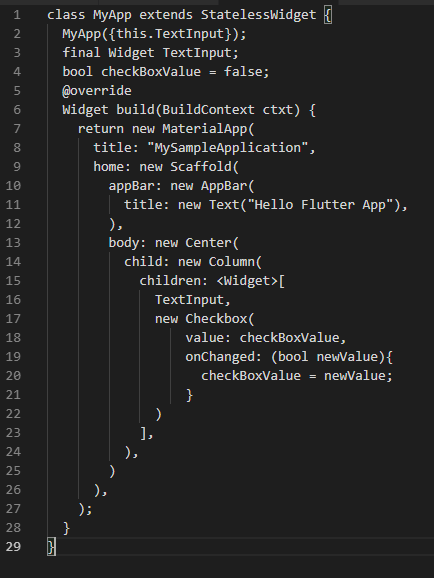
\includegraphics[width=75mm, height=75mm,scale=0.5]{img/stateless.PNG}
\caption{Code sample for stateless widget}
\label{fig:stateless}
\end{figure}

\subsubsection{Stateful Widget}
Stateful widgets are dynamic and have a mutable state. Stateful widgets are widgets which can be read synchronously, when it is created and may change over the lifetime of the widget.\cite{stateful_widgets_2018}. The state can be reloaded by called the setState() method. In order to create a Stateful widget two classes must be made. One of which is created by extending statefulwidget (called myApp) and and another is created by extending the generic state<myApp>(this class is called myAppState). The typical hierarchy structure of a Stateful widget is matericalApp/home/scaffold/body/center/row/column/checkbox.\cite{widgets} \cite{stateful} Stateful widgets idea was originally taken from React Native e.g. the state can not  be changed outside of the state. A real example as to when a stateful widget is used is when having a button on a page such as a like button in order to keep track of how many times this button is pressed by the user the button must be located within a Stateful widget class. \cite{choudhary_2019}


\begin{figure}[ht!]
    \centering
 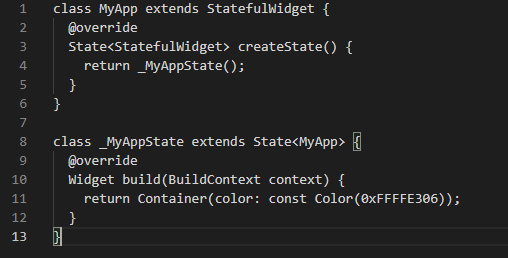
\includegraphics[width=75mm, height=75mm,scale=0.5]{img/stateful.PNG}
\caption{Code sample for stateful widget}
\label{fig:stateful}
\end{figure}

\subsubsection{Inherited Widgets}
An inherited widget is needed when the widget hierarchy gets very large and  information needs to be passed or accessed from a lower branch of the structure. A inherited widget is a widget that can get called directly from any wiget in the tree structure below it. Inherited widgets are ideally kept small for good coding practise.\cite{fidanboylu_2019}.Theme is a type of inherited widget. It can be used in the context theme.of(context).primaryColor. This gets the global theme of a material app. An inherited widget is not able to be changed over time. Similar to stateless widgets they can only be replaced by rebuilding the entire widget.\cite{inherited_widgets}. Inherited widgets have a special unique method called "of". This method can access properties from anywhere on the widget tree.\cite{inheritedwidget_2018}

\subsubsection{Keys}
A key in Flutter is an identifier for widgets and elements. These are rarely used but when used they are ideal for preserving a scroll location and keeping the state when modifying a collection or database.\cite{key_widgets}A to do list application is an example of a time that a key would be useful. Adding, updating, removing and creating items in a collection. Keys are only necessary if the entire sub-tree is stateless. Keys enable the item to be stateful and enables the sub-tree to keep track of the items state when the widget is reloaded. \cite{keys}

\subsubsection{Advantages of Flutter}

\subsubsection{Fast Code Development}
Flutter offers Fast Code Development - this is due to the fact that it is a single code base for both Android and iOS development. This is known as a cross platform framework. All applications developed in Flutter are 2D. Flutter also offers a "hot reload" this enables users to work with developers and easily see changes been made. This hot reload is done in the command prompt which the application is running. Hot reload works by injecting updated source code into the running application on the dart virtual machine.\cite{faq_2019}
\subsubsection{Open Source}
Flutter is an open source framework. It is created by Google and has a large community which means the documentation is extensive and the Dart language is becoming more popular. Flutter has numerous built-in API's to support use of camera, geolocation, network storage and more.\cite{pros_cons}
\subsubsection{Less Code}
There is less actual code to write when using Flutter. Flutter is programmed in Dart. This is an object oriented programming language. Dart has similarities to React-Native because its programming style is reactive and declarative.\cite{pros_cons} Reactive coding ensures only having to declare something once in the code base. This ensures that there is less code to write along with the fact that is becomes more readable and reusable.\cite{depth_flutter_2019}
\subsubsection{Model View Presenter (MVP)}
Flutter is ideal for MVP (Model, View, Presenter) programming pattern. The MVP is replacing the MVC, the controller is exchanged for the presenter. This is a good idea because it enables the developer to create an application to show the customers very fast on both iOS and Android on one code base saving time.\cite{pros_cons}.

\subsubsection{Disadvantages of Flutter}

\subsubsection{Mobile Development alone}
Flutter caters to mobile development alone.(Android and iOS). Flutter is currently unable to create web applications. This is a limitation and may be a reason a company would opt against using Flutter.

\subsubsection{Lack Third party libraries}
Flutter is limited due the amount of third party libraries available to it. This is due to the fact that it is relatively new on the market and is based on Dart.\cite{pros_cons} React-Native has fully extensive third party libraries. It is based on JavaScript so therefore there were already libraries it could use when created. Dart was created by Google also. Therefore it has not developed many external libraries. However these libraries are growing every day. Flutter takes care of User Interface packages needs with widgets. Long term development can be limited.\cite{good_bad}

\subsubsection{Large File Size}
Flutter’s application size is much larger then native applications. The original “hello world” application in Flutter was 6.7mb. After many complaints from developers, the Flutter team managed to reduce the size to 4.7mb. At this, the simple hello world application is still very large in comparison to Java at 539kb and Kotlin at 550kb.\cite{faq_2019} \cite{good_bad}



\chapter{Methodology}
\section{Project Management}

Project Management is a key element of any task to ensure that the project is laid out correctly and each component part is complete at a given date etc. Because this project was completed by a team it was important both members completed each task. In order to track the project a Gantt chart was used. This broke down each step of the project and the expected time limits for each section.

\subsection{Agile}

The project used Agile project management methodologies. An iterative approach was taken. This meant that each week certain tasks are completed. The project team meet 3 times a week to discuss what has been completed since the last meeting, what has to be completed before the next and discuss any difficulties experienced thought out the duration. The meetings are short and concise. Once a week the team met their mentor and explained what was completed since the last meeting and is to be done before the next. These weekly meetings were the iterative approach. Each week the process would be repeated to meet, plan, design, develop, test and evaluate.

\begin{figure}[ht!]
    \centering
 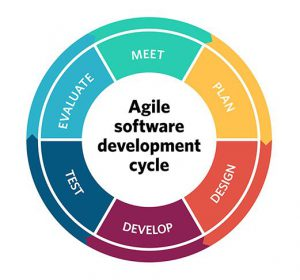
\includegraphics[width=75mm, height=75mm,scale=0.5]{img/agile.jpg}
\caption{Agile Life Cycle}
\label{fig:agile}
\end{figure}

\subsubsection{Agile Roadmap/gantt chart}
An agile Roadmap/gantt chart in agile development to help state the goals of the project from the outset.It helps break down the tasks which are then further broken down for sprints. This is usually a high level view of the project.\cite{testPlan} It is used often in industry and it helps to understand a project as a whole and learn what other teams are contributing to the overall project. The roadmap also shows how the project is likely to show how the project is likely to grow in the future. This is shown to the stakeholders and gives a better indication for funding etc.\cite{roadmap_2016}

\subsubsection{Planning and Development phase}
During the meeting and planning phase, the milestones for the project were identified and broken down into simpler, more manageable tasks. The tasks are then grouped into sprints or iterations lasting one week each (in industry normally 1/3 weeks). These are the tasks which must be be complete before each meeting. Each sprint started after the weekly meeting with the supervisor and the aim is for the work to be complete before the meeting the following week.\cite{Agile}.The plans for the project and the sprints are taken from the user stories. Development iterations convert the iteration plan into working code.\cite{agile_process}

\subsubsection{Design phase}
Throughout the agile development life cycle design is a step in every iteration/sprint. The design is gradually built on. The design is never defined at the beginning of the project. The gradual evolution of the design enables taking advantage of new technologies that come on stream as well as meeting any new requirements brought forward by clients. The user experience is key when designing a project/application. Every design must be user friendly.The type of end user of the item must be considered when designing.

\subsubsection{Testing}
Testing was carried out after multiple iterations. When tasks were complete that were stated in the test plan the tests were carried out. The user tests were carried out when meeting with the client.The client used the applications and commented on any changes that should or could be made.


\subsubsection{Evaluation Phase}
After each sprint before the meeting phase a review was carried out on the tasks completed in the last sprint. If there were changes to make these were completed in the next sprint. In the evaluation section of the agile development cycle the code by both developers was mergers into the master branch of the GitHub repository.The evaluation process is also used to look back, see how much of the previous iteration that was not complete and change the workload applied for a single iteration.\cite{agile_process}


\begin{figure}[ht]
    \centering
 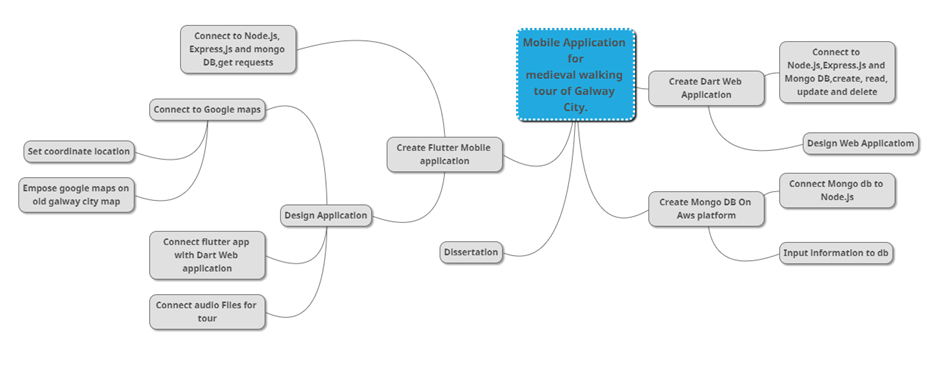
\includegraphics[width=135mm, height=50mm,scale=0.5]{img/plan.png}
\caption{Project Plan}
\label{fig:Project Plan}
\end{figure}

\subsection{Managing Project}
In order to manage this project GitHub was used. This was very useful due to it being a team project. It enables both members of the team to work on separate individual branches. After each iteration, these branches were merged into the master branch. After each integration, the project was at a working state of the project. This could be used for industry standard as continuous delivery. For this project it meant that after each Agile sprint there was a working version to present to customer and supervisor. Although it is a working version is may still need changes in the next sprint. At the beginning of each sprint all branches pull from the master so as every team member is working off the same latest release of code.
\section{System Architecture}
All static text is stored in the MongoDB hosted on url http://35.189.123.3/data. This information is accessed by the Flutter application though the Python code on the Google cloud server which hosts the Mongo database. Each row of the database os called individually to display the appropriate information, update and delete the information.When creating information in the database a new row is added to the end of the database for each entry.The web application both sends and receives information to and from the database while the Flutter mobile application only receives information from the database.
\section{Technologies}
\subsection{Server}
\subsubsection{Mongo and Flask}
To develop the back-end server for the project it was completed using the web framework Flask. It is coded in Python and connected to the MongoDB database. The database was set up in MongoDB on a virtual machine. Google cloud platform was used to host the database containing all the text used in the application. The MongoDB database contains a collection called info. The collection then is made up of documents called id and description. There is an id and description for every location and piece of informative text about the location in the app. The description contains the long pieces of text in the database. The purpose of the id is to decipher each description. The Flask web framework that was set up was also launched on the virtual machine. The same Google cloud virtual machine was used for both the database and the Flask server. 
\paragraph{}Flask was used as a web framework in this case to allow access to the database and display and edit its contents. It can be viewed externally on its own IP address that was created from the VM “35.189.123.3/data?”. This was achieved by connecting MongoDB and Flask to implement CRUD operations. The flask server is run from the ‘index.py’ file. This file contains the route to show the running server. The ‘index.html’ file was used to test that the Flask server could be run of the Google virtual machine. This page is displayed when the IP on its own is searched printing out plain header text. 
\paragraph{}The Flask server was then connected to MongoDB. The PyMongo api allowed the connection between these two frameworks. PyMogno is imported in Flask.  In the ‘init’ Python file it calls the Mongo URI. This allows the recognition of the database. The data types stored in the database are converted to Json string also in this file. This allows readable interpretation of the data. The CRUD implementation in the Flask allows specific routes to access the database. The collection ‘info’ is referenced to ensure the correct data is being accessed. The CRUD functionality is implemented in the Flask through methods Get, Post, Delete and Patch. The Get method does a query to find the id and description. This is accessible through the route data. The IP address allows the route to be added to it ’35.189.123.3/data?’. This IP address will display the contents of the database in JSON string format. This is the read functionality in the CRUD working using the specific method. These methods are programmed in the ‘users.py’ file. The data can then be accessed in the Flutter application and read in to display the data by referencing the IP address. The flask framework lets the data be accessed eternally from a virtual machine, so the data is secure and won’t be lost. 
This framework is used for the create update and delete to allow the data to be edited by the administrator. This is again accessed by the IP address and the look front-end is completed in the index.html. This references the users file and the methods that allow the queries to delete add and update along with the read which is also used in the Flutter application.

\subsubsection{Docker in Flask}
Docker is used on the Debian Virtual machine on Google cloud within the Flask server. The downloads were run and tested inside a Docker container. In the Flask there is a Docker file, this is used in Flask to build a Docker container. It also contains Docker compose files for the development. The Docker file installs all the libraries required and gives flask a port to run off. The port being used is 80.  This is the Google cloud port that can be open to be run externally. The download file makes a Docker container, which defines the network names and ports and the environments being used. The ports 80 are open as you can see in the Docker container file. It also contains the environments that control the Mongo port that it always runs off. This allows in this case the Mongo to be run off a browser and is an external browser. 
\paragraph{}The MongoDB port in the file contains the name of the database that contains the id and description being used. The Docker is run from the command line using docker-compose. This will start the server and run all the libraries and connections. The Docker takes the Python it adds every file of the current directory into the app directory where the container is to be run. Using the Docker allows the web framework to have controlled downloads all in one place. There was less downloads involved, and the imports could be called in the Flask. This also means that if the Flask were to be moved it could be moved to a different virtual machine in one go and will save all the libraries and ports that are needed to connect and run the Mongo ports. The command for Docker compose can then be run from a command line like it is done with this VM and will work in the same way you just use the IP that it is being run off. The files in Flask were generated by themselves when the command lines were run so Docker was easy to set up and the best way to go about the project being on the cloud. 

\subsubsection{Connecting Flutter with the Database}
The text information displayed in the Flutter Application is being stored in the database and not the app itself. The text information is being read into the app from the database, so it is more secure. This was done so the application does not contain large amounts of text. This allowed testing to be done to see how Flutter works with reading from a database as it is a new technology that has not been used in the app development sector. It took a lot of research and testing many different URL readers to fetch the data and be able to display it in the correct way. 
The database was changed many times. In the most recent database, it contains ids and descriptions. Each id is in its own document and is numbered in the database. This allowed for each id to be read in separately so the exact text could be specified in the application.
\paragraph{}This database connection is done in multiple classes in the app e.g. hall.dart, kings.dart, Nicholas.dart. The same string readings are done in the classes. The URL is read in as a string. The URL is of the Data that is displayed in a JSON format when you search the URL.  A method is then used to read any data that is in JSON format. This then will use a set state in the application that reads the data contained in the ‘multi’ document that is in the database. The set state is used to rebuild what the user calls inside it in Flutter.  This means all the data is read in the app to the console. This also decodes the JSON to be able to display it as plain text. To display the text in the app it is completed in the widget. Flutter uses a list view builder. For the data that has been read in to be transferred to the list display an item count is used. This reads the data variable from the json data and add the length of the database. It has been changed to one in this case, so it only reads one piece of information when it is called. A container in the app is what displays the text. The variable is called and has an int and the name of the fields in the database being used. The int is referencing the number each document in the database is given. On the first Hall of the Red Earl page of the app there is a paragraph of text in the database this is in document 20. This can be seen in the container of the MyHallPageState class, it calls 20 and description so will display the correct piece from the database.
\paragraph{}To use the database in an efficient way with Flutter the way the text was being called was changed multiple times. With the research involved the only way it seemed possible to display the text was in a list view. This meant there had to be an integer used in calling the specific pieces of information. This was as the item builder contains the Build context and an int.  Without the list view builder an item builder was not allowed. When the data variable was used with a field from the database it could only print one description as all the data in the collection uses description fields. The data variable had to be used so the text was not being displayed as JSON text.  The data variable could not be used with two fields being called as only one is used in the set state method. This meant this was the only way the data could be displayed in a correct way that suited the database. The containers mean the text is displayed in card like paragraphs that allow for an easy to read display in the application. The text documents and pictures will fit nicely beside each other and the text can be aligned nicely. 

\subsubsection{Web Application}
As part of the project a CRUD web application has been developed for the administrator to edit the data. This was done using the Flask web framework that was set up for running the database from the cloud. The idea was to have a list of options available for the administrator to change the database. They would have been able to add an id and description to the database and edit the information that is in the database by using the id field. There would also be an option to input the id the administrator would want to delete. The remove button would then remove the specific field of the id you were entering. 
\paragraph{}Methods were used to control these in the users.py file. The Get, Post, Delete and Patch were used. To view the page, you can use http://35.189.123.3/view. To view the database, you can click the view button, and this will bring you to the database. It is only viewed as JSON. This is a URL link in the HTML page. It references the user definition This displays the database using a get method. This uses a Mongo query to find the information. The delete function is also working, this is using a post method to delete the information. The delete is done through a MongoDB query in Python code. The edit button is on the page as it is a html page calling the URLs. HTML pages are used to display the information and link the buttons to the definitions which are in the Python file. 

\subsection{Client}

\subsubsection{Mobile Application}
Flutter was used to develop the cross platform mobile application for iOS and Android devices. A lot of research had to be carried out in order to learn dart programming language and learn the syntax of Flutter along with understanding how widgets work correctly. When creating the the applications initially all pages were in one got class. This made the code very long and caused a lot of confusion. At this stage the developers decided to break up the code into a class for each location on the walking tour.

The main page holds the home page of the application along with the splashscreen of the application. The spashscreen widget has an initstate() method. This method calls the timer function which is an async method. The [callback] function is invoked after the given duration passed into the method. In order to display the images on the home page. A widget.dart page was created to hold stateless widgets for each of the images on the main page. These widgets are then called by the main page. The main page imports each of the alternate pages at the top of the class e.g. "import 'package:testing/walls.dart';".
\paragraph{}The maps page contains all elements for the Google maps used within the application. The map view library is imported at the beginning of the file.This enables the creating of a Google maps image in the application. This Google maps image however is places on top of the widget. This was one of the largest problems experienced in the Flutter development of the project. The map view is a separate widget that in linked to directly from Google maps api. This is called from within a stateless widget. When the back button is selected the used is returned to a empty page. For user friendly-ness a message to go back one more page is presented to the user. Flutter has a built in stateless widget called Marker. This enables a specific location to stand out on the map and when clicked a label appears over the marker. The Marker method takes the parameters (String id, String title, double longitude ,double latitude).The maps page is called by each of the location pages.
\paragraph{}Each page containing the locations of the tour are laid out in similar format. Each file contains 2 stateful widgets. One of these is the initial page for the location. This page contains multiple photos in a scrolling slide show. This user must select previous/next button to navigate though the images. The images are stored in a list and list is controlled by a photo Index to see what number of the list is currently being displayed. The text for each page is taken directly from the MongoDB Flask database. The url location that the information from the database. The second stateful widget contains more detailed information about each location. This information was provided by Galway Civic Trust and is based on the information in "Galway City medieval walk" booklet available at the Hall of the Red Earl. The images included in this booklet are also in the application in similar format.


\section{System Integration}
Due to this project being produced in conjunction with Galway Civic Trust, working closely with Michael Quinn to produce the exact item he wished to publish is necessary. In order to do this Software Engineering techniques are being used to ensure the customer receives exactly what’s needed. The main approaches used are test driven development (TDD), behaviour driven development (BDD) and user storyboards.

\subsection{Storyboards}

Storyboards were used to allow the customer give the developer’s a high level view of expected design of the application. This is done using a blank page and the customer draws a simple representation of what they want the application to look like. This gives the developers a better understanding and idea what needs to be done and can help break down upcoming tasks to be completed. The storyboard used is taken from the agile methodology and is continuously being referred to and brought to each meeting with the customer to ensure every design requirement is clearly met. \cite{StoryBoard}

\subsection{Behaviour Driven Development}

Behaviour driven development is another agile software development methodology. It is designed based on what the user wants and how the user explains what the visual display of the application should look like. The customer/user gives a list of behaviours they wish the application be able to accomplish. These simple requests become a task or multiple tasks for the developer. When the application is complete the original requirements are made into unit tests.\cite{BDD} 

\subsection{Test Driven Development}

Test Driven Development is based predominantly on unit testing. However they are very different because test driven development is when the unit tests are written before the code has been created. This means the developers are using the unit tests as a guild and the tests alone break down the overall task needing to be completed. The tests will initially fail and the developers write minimal code in order for the tests to pass. This is process in continuously repeated in order for the application to pass each test. These tests are commonly automated.\cite{TDD}

\chapter{Results}

\section{Testing}
Testing is an essential part of any software development life cycle. The importance of testing in software development life cycle is to improve reliability, performance and other important factors.\cite{TestingLifeCycle} Each component of the project can be tested individually.

\subsubsection{Test Plan}
A test plan consists of a list of scenarios and exact instruction of what needs to be tested in a project. The test plan must state exactly the features that need to be tested, the method in which they will be tested, the order these tests should be carried out and a time frame for these tests. The time frame ensures that testing is not left too late in the product life cycle.\cite{testPlan}
 
\subsubsection{Unit Tests}

Unit tests are individual tests to check functions, methods or classes. A test library is imported into the Flutter application. The developer/tester can run the unit tests from the terminal to check for success or failure. Unit tests can test that visual aspects of the application are working correctly along with connection to the backend database.

\subsubsection{Widget Testing}

A widget test exercises a single widget. Testing a widget involves multiple classes and requires a test environment that provides the appropriate widget life cycle context. \cite{testing}. It tests that the widget user interface performs as expected both visually and in it’s interactions. A widget should be able to check for user input and check for responses for the user based on actions performed. It is similar to unit testing because it tests the environment and is usually created to test certain actions alone.

\subsubsection{Integration Testing}

Integration testing is used to test the Flutter application as a whole. This tests that each function checked in unit and widget tests also work when incorporated with the remainder of the application. Integration testing is also used to test the performance of the application. This was done to test that the application could retrieve information from the database by many users simultaneously. Developers/testers can run the command "Flutter driver" which sets up the test harness, builds and installs the application and runs the integration tests on the application. \cite{IntegrationTest}

\subsubsection{Fuzz Testing}
In order to carry out tests on the web application and Mongo database, fuzz testing is used. This means testing the architecture by giving it a large variety of inputs. The web application updates, creates and deletes inputs from the MongoDB. The input size is limited and this limit is tested to the max though fuzz tests, along with invalid inputs such as no input and numeric input alone. This testing is to be completed after the basic level of testing.

\begin{figure}[ht!]
    \centering
 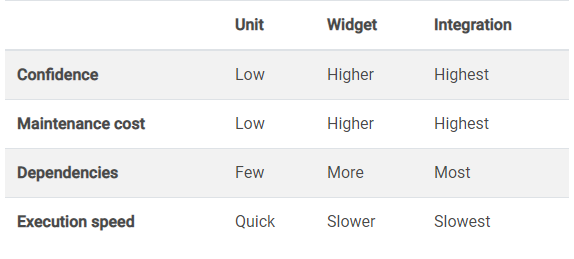
\includegraphics[width=125mm,scale=0.5]{img/Capture.PNG}
\caption{Testing:Types of testing}
\cite{testing}
\label{fig:method}
\end{figure}

\section{Complications}


\subsection{Flutter Complications}
When creating the mobile application multiple problems were encountered. Many steps did not work as initially planned.
\subsubsection{Learning Flutter}
Learning Flutter from basics was the first difficulty faced by the developers. However because Flutter is built by Google there are many open source online video and articles which help the learning process. Because of the developers knowledge of object oriented programming languages such as Java it reduced the learning curve of Flutter. However Flutter's widgets took longer than expected to fully understand and know when/how to use.
\paragraph{}When Beginning the learning process of Flutter the first place the developers looked was the Flutter docs.\cite{flutterdocs} The official documentation Flutter has provided for its developers is very good.It includes easy step by step examples of nearly every favourable scenario. The documentation is broken up into "Flutter for Android devs", "Flutter for iOS devs" , Flutter for react native devs", "Flutter for web devs".This breakdown enables developers to relate to Flutter from different perspectives based on previous knowledge. The developers also came across a Youtube channel called MTechViral.\cite{channel_youtube} This channel posts videos on mobile development and have a Flutter playlist. This YouTube channel is very popular and therefore a great place to communicate to other developers and learn from their experiences also.

\subsubsection{Incorporating Google maps}
There was a lot of research put into incorporating Google maps into the application correctly.When the developers began this process there was limited documentation on Google maps integration to Flutter applications.
\paragraph{}In order to incorporate Google maps into the application, there are multiple steps that must be followed.In order to use Google maps within a Flutter application,the \texttt{google\_maps\_flutter} plugin must be added as a dependency in the pubspec.yaml file of the application.Each developer must get a unique api key from Google cloud platform.\cite{googleCloudMap}.The api key must be identified in the Android application manifest and the iOS application delegate. The Google maps plugin allows the Googlemap widget be added to a widget tree and map view is controlled by the Google maps controller. This however has limitations, there are no markers supported.
\paragraph{}
The map attempted is \texttt{map\_view} plugin however this was not ideal due to the fact that is open the map within the application page but instead create a page ontop of the page and in order to go back to the previous page the user must press the back button on an adroid device or manually shut the application on an iOS device. This was not very user friendly.A toolbar Action page has been added to ensure the ability to go back to the previous page.This is not working currently.

\subsubsection{Navigation between pages}
Flutter is unique with its use of widgets. In order to navigate between pages of a Flutter application there must exist two or more routes. To switch to a new route the navigator.push() method must be called. This allows the new route to be added to the stack of routes managed by the navigator. In order to return to the previous route of an application the navigator.pop() method is called. This method removes the current route from the stack. In order to access a route that is in a different .dart file the correct file containing the route must be imported at the top of the .dart page.

\subsubsection{Flutter Version Conflicts}
Throughout the development process of this application there have been many new releases by Flutter. The development began on Flutter version 0.8. The finished version of this project was completed on version 1.3.4. Because this project was carried out in a group it is important that all developers are on the same version of Flutter, dart, framework and engine. When running the command "Flutter upgrade the correct updated versions should be installed with the correct libraries. This was a problem faced one developer was a version behind. This led to problems with libraries included and package version conflicts. This issue was resolved by instead of stating specific versions of an item e.g.http in the pubspec.yaml the version was resolved to any.

\subsection{Back-end Conplication}
The database and backend server were first set up with NodeJS. The MongoDB database was set up alongside this and deployed on the Google Cloud Platfrom. The virtual machine was a windows version. NodeJS was being used to run and display the MongoDB database. The database contained one id and one description to test. The html webpage was run locally on a Google cloud platform virtual machine. It was also accessible externally by an IP address. The ports for Google Cloud Platform were open so it was accessible remotely these ports were ports 80 and 3000. The page displayed just plain text placed in a header. The Mongo database was then connected to this framework. It used Mongo's URL and default port 27017 to connect and run it from the browser. When the node was run from the command line it was displayed that the JS and Index were connected to the database. 

\subsubsection{Issues with NodeJS}
By connecting the JavaScript to the Mongo and port 3000 it was able to run from the URL. When this was run it was displaying invalid information. The connection was working as the page was printing back empty brackets. This meant the database could be recognised but the information inside the database could not be correctly read by NodeJS. Research was done as to how to fix this error. The database was then changed and the names in the JavaScript were changed around to get the information displaying. MongoDB was used to test the database and that the collection was implemented correctly. This issue was not with the data and how it was inserted into the database. The code was error tested that if the database was not connecting it would print error, when the database was connected and printing it told the user so. This line did print in the console along with the empty brackets in the browser. The fact the data could not be retrieved meant an application could not be connected to the specific IP for access to the database in order to read in information.
\paragraph{}NodeJS was nice and easy to use when it came to setting up a webpage to be accessed from the browser remotely on Google Cloud Platform. After much research and testing the correct data needed could not be viewed in the browser. The issue with the database took time to fix and, in the end, it was changed to MongoDB with Flask to access the data remotely.

\subsubsection{Problems with the CRUD Web Application}
When viewing the data this was not the intended way. There were difficulties when trying to connect the id and description to the Python and HTML. The only way it was possible to view the data was to link it to the JSON display page. The delete button removed information from the database. It is not deleting the specific id that is being entered. It is deleting the first field in the database when the button is pressed. This is not the correct way for the administration page to work. This is then deleting data from the database that is needed for the application. The edit and add functions are not working. The code is in the Flask in the Python files to show how the functions worked. Due to time limitations this was not possible to get the add and edit working to any extent. The HTML connections were the biggest problem with the Flask. The ObjectId in the Python was not connecting to the fields in the database which was causing a problem with connecting the HTML and the Python in order to recognise the id field. There was a lot of research done to run a CRUD web application but there was not time to start another framework and it was better to use Flask as this was set up with the database previously. This was a major issue with this project. The read function was completed within the Flutter application. The CRUD was an extra feature for the project just to implement CRUD. This would be a further development for the project that would be a helpful function in a project that contains a database.

\subsection{Screenshots}

\begin{figure}[ht!]
    \centering
 
\includegraphics[width=75mm,height=162mm]{img/splashscreen.jpg}
\caption{SplashScreen}
\label{fig:Splash screen of application}
\end{figure}

\begin{figure}[ht!]
    \centering
 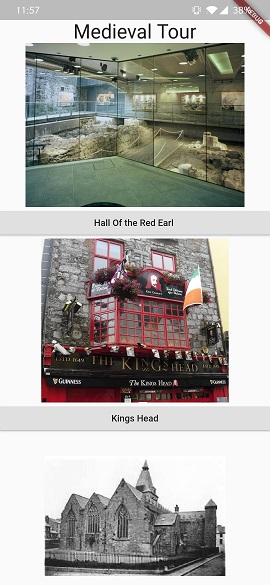
\includegraphics[width=75mm,height=162mm]{img/homeshot.jpg}
\caption{Home Page}
\label{fig:Home page of mobile application}
\end{figure}

\begin{figure}[ht!]
    \centering
 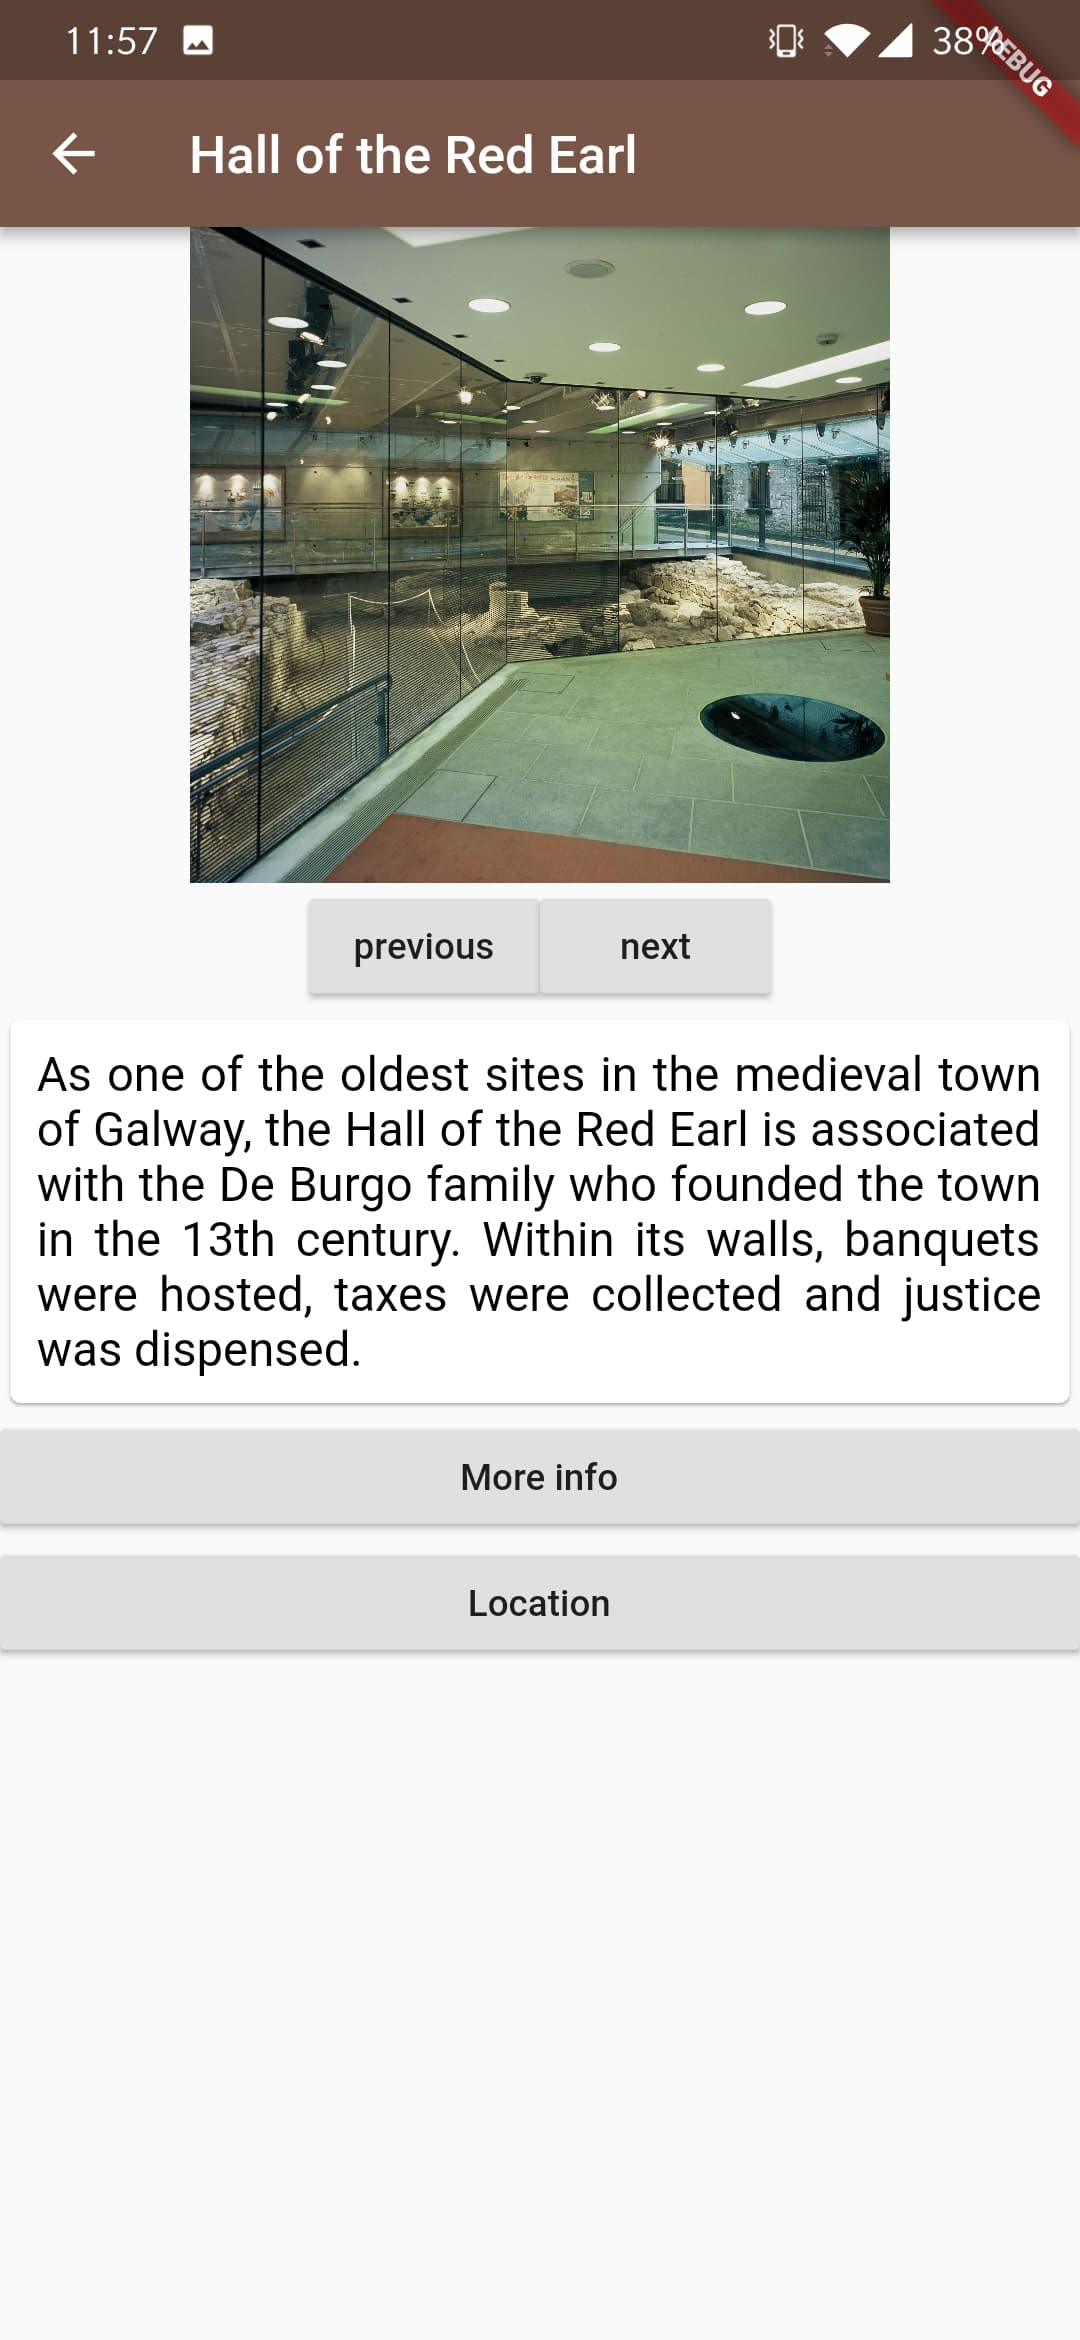
\includegraphics[width=75mm,height=162mm]{img/HallRedEarl.jpg}
\caption{Hall Of the Red Earl}
\label{fig:Hall Of the Red Earl}
\end{figure}

\begin{figure}[ht!]
    \centering
 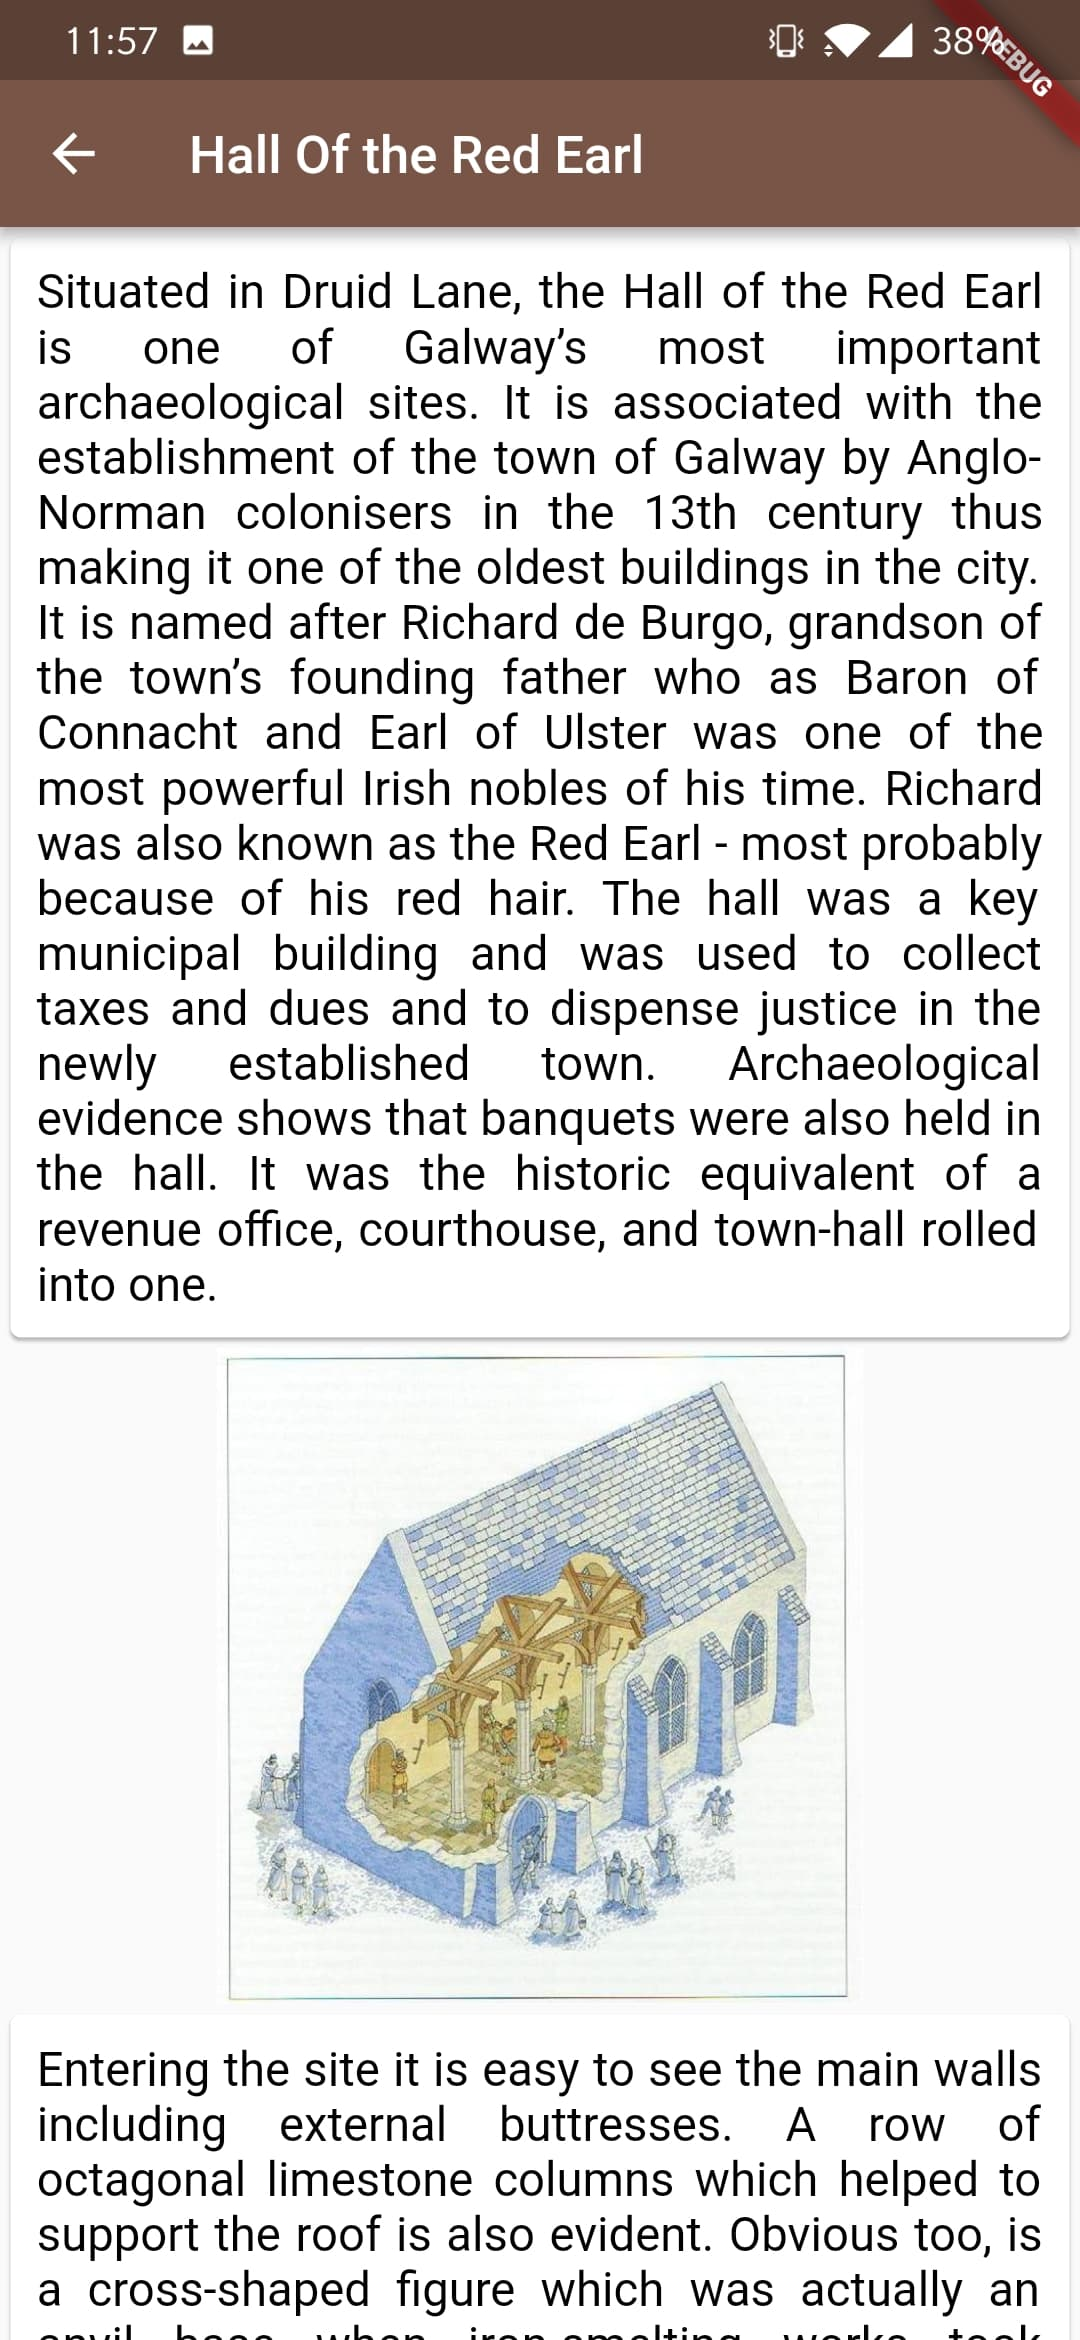
\includegraphics[width=75mm,height=162mm]{img/HallRedEarlMore.jpg}
\caption{Hall Of the Red Earl more}
\label{fig:Hall Of the Red Earl more}
\end{figure}

\begin{figure}[ht!]
    \centering
 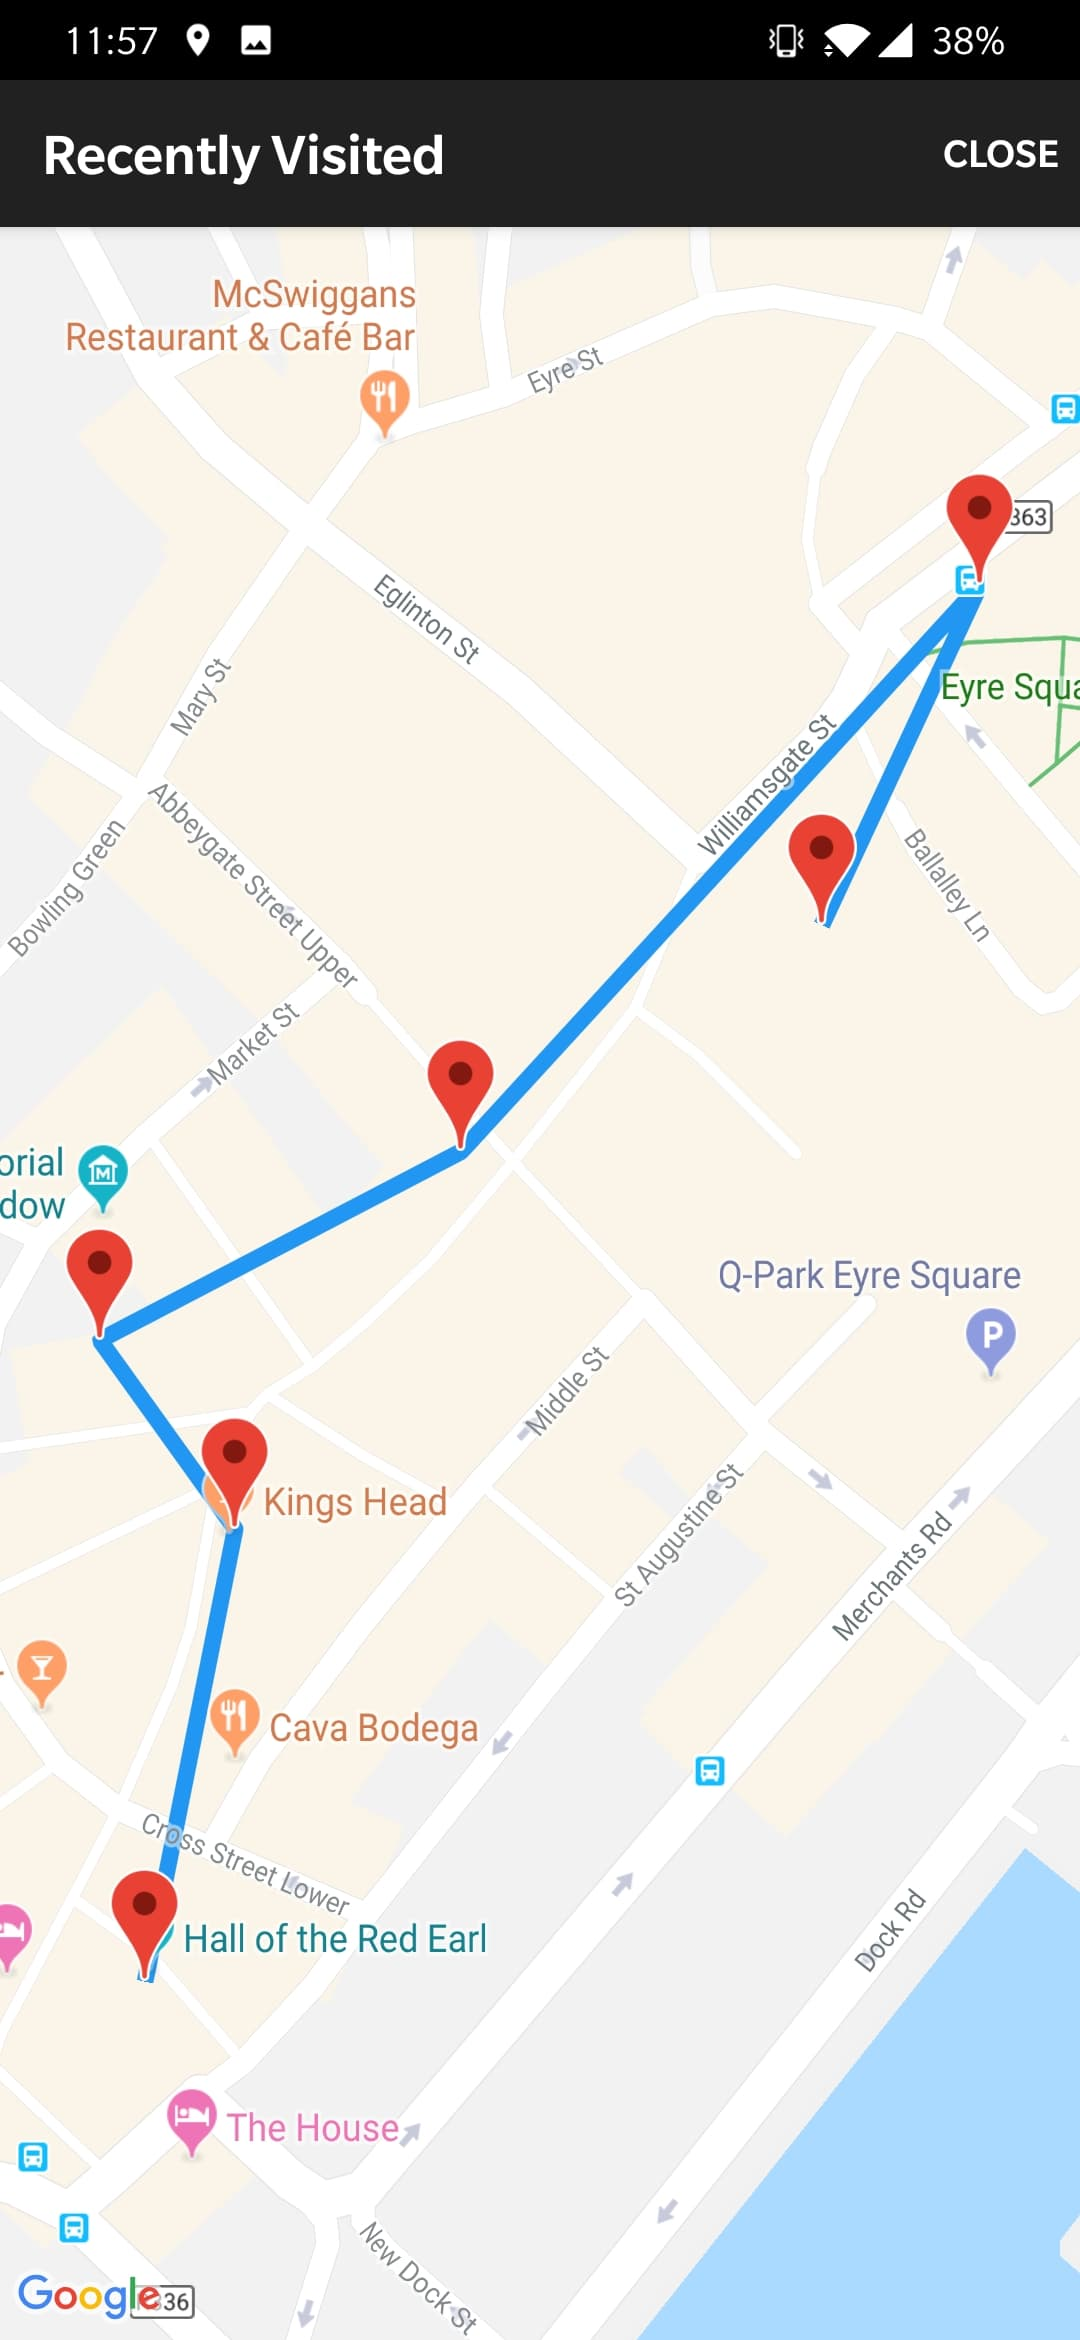
\includegraphics[width=75mm,height=162mm]{img/Markers_polyline.jpg}
\caption{Map displaying markers and polyline}
\label{fig:Map displaying markers and polyline}
\end{figure}

\begin{figure}[ht!]
    \centering
 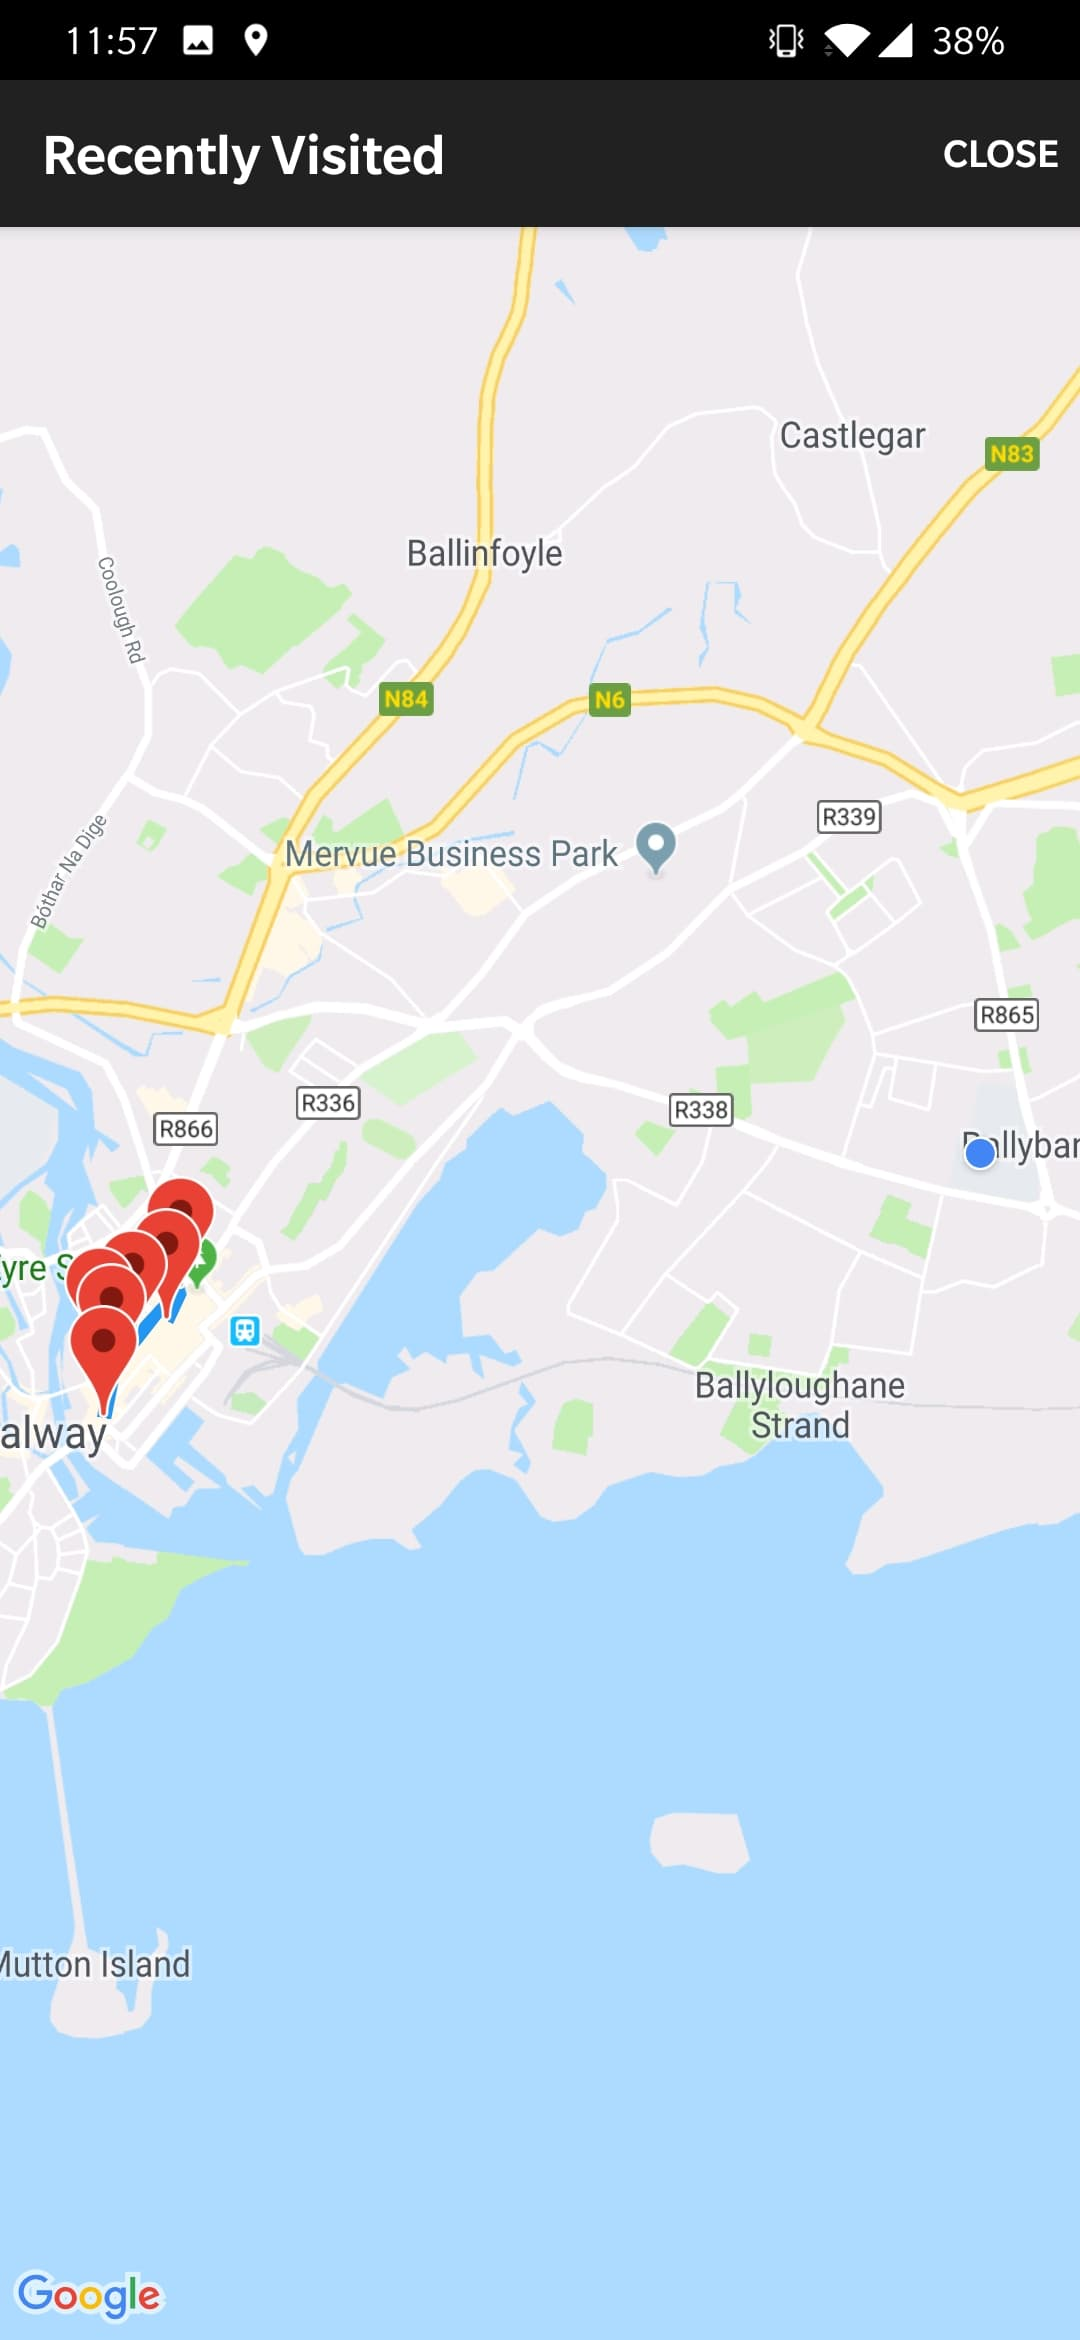
\includegraphics[width=75mm,height=162mm]{img/map_currrentLocation.jpg}
\caption{Map displaying markers and users Location}
\label{fig:Map displaying markers and location of user}
\end{figure}


\chapter{Conclusion}
Writing this document and developing the project signals the areas that were completed in an easy way and the areas that caused the most issues. The research completed was helpful in deciding what frameworks and platforms were best to use in completing a functioning application for users and back-end server. Throughout the document it gives detailed process of the work involved in completing the project to a high standard. The objectives described at the start of the project have all been covered in the methodologies or the complications section of the project. 
\paragraph{}A back-end server was set up to connect the Flutter application to the database. A GPS Application was set up showing the users location and the locations of the historical sites. The web Client was not completed in the intended way, but this has been documented explaining the issues. The Technology Sections gives detailed research of the technologies like the ones used in completing the project. It gives a clear comparison of these technologies and how they are similar and differ in some ways. The background section in this section gives information about the technologies chosen. This helps understand why these specific technologies were chosen and why they suited our project. All testing involved in the development of the project is also documented to get a full view of the steps involved.
\paragraph{}Flutter was a new technology that was used to develop an application. There was many issues using this technology as it is still in early stages of development. The mobile application was easy to deploy on phones for testing which was a feature that was enjoyable. MongoDB and Flask was a new technology that is now up and coming in the technology sector. This was also difficult as there were not many ways of finding information on the issues that emerged.
\paragraph{}As the Application was developed for a local enterprise it meant the application had to meet the standards of the collaborator. The meetings were successful, and the application was changed if there were any issues and completed in the way that it was intended for the user. The Application was one that had not been completed before for Galway which meant it was an original application.
\paragraph{}The time limitations were the main issue with the project. This means that in future there would need to be more time spent on the web application in order to set up the administrator’s page in order to edit the database in an easy way. The research and development meant a lot of time and detail went into this project to complete a functioning Application and Back-end server.
